\begin{figure}[htb]
\centering
\includegraphics[page=6,width=0.45\textwidth]{\FCNCFigures/tthML/raw/faketau/prefit/NOMINAL/reg1l1tau1b2j_os/tau_pt_0.pdf}
\put(-100, 140){\textbf{(a1)}}
\put(-120, 130){\footnotesize{$STH \tlhad OS$}}
\includegraphics[page=6,width=0.45\textwidth]{\FCNCFigures/tthML/raw/faketau/prefit/NOMINAL/reg1l1tau1b2j_ss/tau_pt_0.pdf}
\put(-100, 140){\textbf{(a2)}}
\put(-120, 130){\footnotesize{$STH \tlhad SS$}}

\includegraphics[page=6,width=0.45\textwidth]{\FCNCFigures/tthML/raw/faketau/prefit/NOMINAL/reg1l1tau1b3j_os/tau_pt_0.pdf}
\put(-100, 140){\textbf{(b1)}}
\put(-120, 130){\footnotesize{$TTH \tlhad OS$}}
\includegraphics[page=6,width=0.45\textwidth]{\FCNCFigures/tthML/raw/faketau/prefit/NOMINAL/reg1l1tau1b3j_ss/tau_pt_0.pdf}
\put(-100, 140){\textbf{(b2)}}
\put(-120, 130){\footnotesize{$TTH \tlhad SS$}}

\includegraphics[page=6,width=0.45\textwidth]{\FCNCFigures/tthML/raw/faketau/prefit/NOMINAL/reg1l2tau1bnj_os/tau_pt_0.pdf}
\put(-100, 140){\textbf{(c1)}}
\put(-120, 130){\footnotesize{$l\thadhad OS$}}
\includegraphics[page=6,width=0.45\textwidth]{\FCNCFigures/tthML/raw/faketau/prefit/NOMINAL/reg1l2tau1bnj_ss/tau_pt_0.pdf}
\put(-100, 140){\textbf{(c2)}}
\put(-120, 130){\footnotesize{$l\thadhad SS$}}

\caption{ The data-MC comparison of $\tau$ $\pt$ in the signal and SS control regions. }
\label{fig:pt_raw}
\end{figure}
